\documentclass[sigconf,review]{acmart}
\setcopyright{none}
\settopmatter{printacmref=true}
\acmConference[WWW '27]{ACM Web Conference 2027}{May 10--14, 2027}{Dublin, Ireland}
\acmYear{2027}
\acmDOI{}
\acmISBN{}
\usepackage{booktabs}
\usepackage{amsmath}
\usepackage{graphicx}
\usepackage{tikz}
\usetikzlibrary{arrows.meta}
\title{Preserving Visual Evidence While Repairing Industrial Diagram Graphs}
\author{Minhyeong Yu}
\email{minhyeong@enhans.ai}
\affiliation{\institution{Enhans}\city{}\country{}}
\author{Seunghyun Lee}
\email{seunghyun@enhans.ai}
\affiliation{\institution{Enhans}\city{}\country{}}
\renewcommand{\shortauthors}{Yu and Lee}
\begin{document}
\begin{abstract}
Raster industrial diagrams encode relationships that text indexing cannot recover. We study an evidence-bearing extraction framework combining geometric proposals, legend-conditioned paired Decision Model judgments, bounded body repair, and original-pixel connection checks. We formalize its decision rules and distinguish direct edges, containment, and within-net reachability in a separate frozen-output audit. We evaluate two unchanged extractor revisions on all 12 real OPEN100 plans in the public PID2Graph benchmark, using only public synthetic exemplars and class descriptions. Against 1,439 annotated symbols, the candidate achieves 51.71\% precision, 21.06\% recall, and 29.93\% F1 at IoU $\ge .50$. Adapted symbol-net connectivity yields 22.49\% precision, 7.01\% recall, and 10.69\% F1 over 1,882 reference pairs. Only two plans pass strict output preservation; 14 mapped direct pairs and 57 mapped within-net pairs are lost. Original-crop examples expose both correct and missed connections. The public evaluation establishes substantial transfer limitations rather than a general repair or preservation guarantee.
\end{abstract}
\begin{CCSXML}
<ccs2012>
<concept><concept_id>10010147.10010178.10010219</concept_id><concept_desc>Computing methodologies~Image processing</concept_desc><concept_significance>500</concept_significance></concept>
<concept><concept_id>10002951.10002952.10002953</concept_id><concept_desc>Information systems~Information retrieval</concept_desc><concept_significance>300</concept_significance></concept>
</ccs2012>
\end{CCSXML}
\ccsdesc[500]{Computing methodologies~Image processing}
\ccsdesc[300]{Information systems~Information retrieval}
\keywords{diagram understanding, graph extraction, visual verification, provenance}
\maketitle

\section{Introduction}
Industrial drawings encode device connections that text indexing leaves implicit. Extraction must turn pixels into inspectable graph facts with supporting evidence. A detected gate may omit its input bar, a motor rim may be clipped, and enlarging a body can obscure its short output neck in a whole-pair view. Local repairs may also alter earlier outputs.

\paragraph{Relevance to the Web.}
Knowledge graphs organize entities and relationships~\cite{hogan2021knowledge}; provenance records their derivation~\cite{buneman2001provenance,lebo2013provo}. Raster engineering archives supply document-bound knowledge. Here, accepted relationships retain original paths and judgments, and revision audits expose lost facts. Web integration motivates acquisition, but RDF services and retrieval are not evaluated.

We combine constrained geometric repair, paired visual checks, and a separate preservation contract, distinguishing direct edges, reference-matchable endpoint pairs, and within-net reachability. Public evaluation reveals missed symbols and failed preservation; the audit reports those failures without certifying correctness.

\section{Related Works}
Engineering-diagram digitization combines recognition and graph search for equipment mapping and diagram search~\cite{mani2020digitization}. Digitize-PID extracts P\&ID components and connections and provides synthetic evaluation data~\cite{paliwal2021digitize}; transformer-based extraction introduces PID2Graph with graph annotations~\cite{sturmer2025pid2graph}. Our focus is repair with source evidence and preservation across frozen revisions.

AI2D provides constituent and relationship parse graphs for educational diagrams~\cite{kembhavi2016diagram}, an auxiliary domain rather than an industrial topology test. POPE studies object hallucination in visual-language models~\cite{li2023pope}. Our Decision Model controls original-pixel checks; its trace records locations and decisions without certifying semantic truth or implementing formal database provenance or PROV-O. External-system comparison remains unperformed.

\begin{figure*}[t]
 \centering
 \resizebox{\textwidth}{!}{\begingroup
\definecolor{cadnavy}{HTML}{233D5B}
\definecolor{cadteal}{HTML}{187A77}
\definecolor{cadred}{HTML}{B83F4B}
\definecolor{cadblue}{HTML}{3473B8}
\begin{tikzpicture}[
 x=1cm,y=1cm,
 font=\sffamily\fontsize{8}{9.2}\selectfont,
 head/.style={font=\sffamily\bfseries\fontsize{8.5}{9.5}\selectfont,text=cadnavy,anchor=west},
 note/.style={font=\sffamily\fontsize{7.5}{8.5}\selectfont,align=center},
 flow/.style={-{Stealth[length=3.8pt,width=3.8pt]},draw=cadnavy,line width=.75pt},
 ink/.style={draw=black!80,line width=.7pt},
 crop/.style={draw=black!25,fill=white,line width=.45pt},
 port/.style={fill=cadteal,draw=white,line width=.3pt},
 auditflow/.style={-{Stealth[length=3pt,width=3pt]},draw=black!45,line width=.5pt}
]
\path[use as bounding box](0,0)rectangle(17.7,3.52);
\foreach \xx in {0,3.6,7.2,10.8,14.4}{
 \draw[cadteal!70,line width=1.05pt](\xx+.05,3.02)--(\xx+3.25,3.02);
}
\node[head]at(.08,3.25){(a) Prepare \& propose};
\node[head]at(3.68,3.25){(b) Fit \& classify};
\node[head]at(7.28,3.25){(c) Propose connections};
\node[head]at(10.88,3.25){(d) Verify connections};
\node[head]at(14.48,3.25){(e) Text \& export};

% (a) The raster is searched for candidates before any class/box judgment.
\draw[crop](.35,1.72)rectangle(2.95,2.78);
\draw[black!55,line width=.55pt](.54,2.17)--(.84,2.17);
\draw[ink](1.10,2.17)circle(.26);
\draw[ink](1.36,2.17)--(1.83,2.17);
\draw[ink](1.83,1.98)--(2.21,2.36)--(2.21,1.98)--(1.83,2.36)--cycle;
\draw[ink](2.21,2.17)--(2.72,2.17);
\draw[cadteal,line width=.75pt](.77,1.84)rectangle(1.43,2.50);
\draw[cadteal,line width=.75pt](1.73,1.87)rectangle(2.31,2.47);
\node[note,text=black!60]at(1.65,1.48){raster $X$ $\rightarrow$ candidate boxes};

% (b) Two existing boxes are compared; the retained class survives repair.
\foreach \xx in {4.42,6.07}{
 \draw[crop](\xx-.54,1.87)rectangle(\xx+.54,2.76);
 \draw[black!50,line width=.7pt](\xx,2.31)circle(.27);
 \draw[ink](\xx+.27,2.31)--(\xx+.47,2.31);
}
\draw[black!55,line width=.75pt](4.22,2.11)rectangle(4.62,2.51);
\draw[cadteal,line width=.9pt](5.74,1.98)rectangle(6.40,2.64);
\node[note]at(4.42,1.68){$b_1$};
\node[note]at(6.07,1.68){$b_2$};
\draw[draw=cadnavy,<->,line width=.65pt](4.98,2.30)--(5.49,2.30);
\node[note,text=black!60]at(5.25,1.46){box alternatives; class $c_i$};

% (c) Geometry produces a net, its ports, and source-pixel route hypotheses.
\draw[ink](7.89,2.12)--(9.81,2.12);
\draw[ink](8.85,2.12)--(8.85,2.55);
\foreach \xx/\yy in {7.70/2.12,10.00/2.12,8.85/2.74}{
 \draw[black!45,fill=white,line width=.6pt](\xx,\yy)circle(.19);
}
\foreach \xx/\yy in {7.89/2.12,9.81/2.12,8.85/2.55}{
 \draw[port](\xx,\yy)circle(.05);
}
\node[note]at(7.70,2.12){$u$};
\node[note]at(10.00,2.12){$v$};
\node[note]at(8.85,2.74){$w$};
\node[note,text=black!60]at(8.85,1.48){hypothesis $(u,v,n,\pi)$};

% (d) Both presentations retain the source ink and exchange endpoint colors.
\foreach \xx/\name/\lc/\rc in {11.04/A/cadred/cadblue,12.65/B/cadblue/cadred}{
 \draw[crop](\xx,2.08)rectangle(\xx+1.39,2.74);
 \draw[ink](\xx+.23,2.40)circle(.10);
 \draw[ink](\xx+1.16,2.40)circle(.10);
 \draw[ink](\xx+.33,2.40)--(\xx+.62,2.40)--(\xx+.62,2.52)--(\xx+1.06,2.52)--(\xx+1.06,2.40);
 \draw[\lc,line width=.85pt](\xx+.08,2.25)rectangle(\xx+.38,2.55);
 \draw[\rc,line width=.85pt](\xx+1.01,2.25)rectangle(\xx+1.31,2.55);
 \node[note]at(\xx+.695,1.90){\name};
}
\node[note,text=cadnavy]at(12.45,1.48){paired scores; local evidence};

% (e) A text-to-symbol containment relation remains distinct from the edge.
\draw[cadnavy,line width=.9pt](15.12,2.32)--(17.01,2.32);
\foreach \xx/\name in {15.12/u,17.01/v}{
 \draw[ink,fill=white](\xx,2.32)circle(.23);
 \node[note]at(\xx,2.32){$\name$};
}
\node[crop,minimum width=.37cm,minimum height=.25cm,inner sep=1pt]at(15.12,1.70){$t$};
\draw[flow](15.12,1.84)--(15.12,2.07);
\node[note,anchor=west]at(15.34,1.93){$I$};
\node[note,text=cadnavy]at(16.42,1.65){$\mathcal G=(V,E,I,\rho)$};

% Only the five major outputs are connected: no long return or bypass arrows.
\foreach \xa/\xb in {3.28/3.56,6.88/7.16,10.48/10.76,14.08/14.36}{
 \draw[flow](\xa,2.32)--(\xb,2.32);
}
\node[note]at(1.65,1.03){Preprocess $\rightarrow$ S0$^*$ $\rightarrow$ S1\\Geometry $\rightarrow$ S2};
\node[note]at(5.25,1.03){B6$^*$ $\rightarrow$ deduplicate $\rightarrow$ C1\\C2$^*$ $\rightarrow$ repair / cleanup};
\node[note]at(8.85,1.03){Body mask $\rightarrow$ nets $\rightarrow$ ports\\BFS / tree $\rightarrow$ pair proposals};
\node[note]at(12.45,1.03){K3: global acceptance\\K5$^*$ / K6$^*$: review or recovery};
\node[note]at(16.05,1.03){Text candidates $\rightarrow$ T1 $\rightarrow$ T2$^*$\\Text geometry $\rightarrow$ $I$ $\rightarrow$ export};
\node[note,anchor=west,text=black!60]at(.10,.56)
 {$^*$ Conditional call; question IDs and panel letters are distinct. Exact scope follows in the matching Method subsection.};

% (f) Retention audit is visibly separate and consumes saved graphs only.
\draw[black!25,line width=.45pt](.05,.35)--(17.65,.35);
\node[head,font=\sffamily\bfseries\fontsize{8}{9}\selectfont]at(.08,.13){(f) Offline audit};
\node[note]at(4.30,.13){saved old + new graphs};
\node[note]at(8.33,.13){object correspondence $f$};
\node[note]at(12.28,.13){compare $E$, $I$, within-net $R$};
\node[note]at(16.05,.13){retained / lost / unmapped};
\draw[auditflow](2.50,.13)--(2.96,.13);
\draw[auditflow](5.78,.13)--(6.68,.13);
\draw[auditflow](9.97,.13)--(10.54,.13);
\draw[auditflow](14.02,.13)--(14.41,.13);
\end{tikzpicture}
\endgroup
}
 \caption{Evidence-grounded extraction. Panels match the Method subsections; (f) independently audits saved graphs. S/B/C/K/T are question IDs; $^*$ marks conditional calls. Drawings are implementation schematics.}
 \Description{Five left-to-right panels each show a simple schematic and the corresponding question identifiers. Panel a prepares the raster and proposes candidate boxes using S0, S1, geometry and S2. Panel b compares existing body boxes, assigns legend classes using B6, C1 and selected C2, and repairs the retained body without changing its class. Panel c shows a traced net and boundary ports, from which code creates candidate endpoint pairs and routes. Panel d shows identical source views with red and blue endpoints swapped for K3; K5 and K6 provide conditional local and endpoint checks. Panel e exports an accepted edge and a separate directed text containment relation, after T1, selected T2 and text geometry. The lower, disconnected lane f compares saved old and new graphs via object correspondence and reports retained, lost and unmapped direct edges, containment and within-net reachability. Stars mark conditional question calls, whose precise scope is explained in the matching Method subsections.}
 \label{fig:framework}
\end{figure*}

\section{Method}
\label{sec:method}
Given grayscale raster $X\in\{0,\ldots,255\}^{H\times W}$ and a fixed legend, the framework exports $\mathcal G=(V,E,I,\rho)$. Vertices store inclusive full-resolution boxes and symbol-class keys (possibly unset) or \texttt{text}; $E$ stores undirected exterior connections and $I$ directed text-to-symbol containment. The trace $\rho$ retains source paths and decisions. Figure~\ref{fig:framework}(a)--(e) follows extraction; (f) is a separate audit. The following subsections use the same letters and titles. The Decision Model answers original-crop questions with fixed choices or binary scores; no fine-tuning is performed. Question IDs such as S2 and B6 are not version numbers.

\subsection{(a) Prepare and Propose}
\label{sec:prepare}
Code removes the page frame and coordinate strips, detects ruled tables, and scales thresholds by estimated letter height. S0 selects CLD or P\&ID unless the kind is configured; S1 identifies diagram regions. Contour holes, filled components, open-shape rules, and structured merging then propose boxes. S2 judges original candidate crops as symbols, fragments, or other content. Its retained candidates enter panel (b); the model does not generate their coordinates.

\subsection{(b) Fit and Classify}
\label{sec:fit}
For each retained candidate, code constructs an outline box and a protected extension enclosing attached body strokes. B6 compares original-image views in swapped orders if the maximum coordinate difference is at least two pixels. Code deduplicates the selected boxes; C1 assigns a key from the fixed legend of descriptions and optional exemplars. Selected ambiguous bodies receive C2 detail review, including P\&ID closed-box checks. Available B6/C1 categorical answers are remapped to shared labels:
\begin{equation}
 \bar p_q(c)=|\mathcal A_q|^{-1}\sum_{a\in\mathcal A_q}p_q^a(c),
 \qquad \varnothing\ne\mathcal A_q\subseteq\{A,B\}.
 \label{eq:cat}
\end{equation}
B6 selects an existing box. C1 takes the highest non-\texttt{other} score, unless $\bar p_q(\texttt{other})\ge .50$ and S2 support is below .40 for P\&ID (whole symbol) or .70 for CLD (whole plus part). For $n>1$ legend choices, confidence is $\gamma(p,c)=\max\{0,(p(c)-1/n)/(1-1/n)\}$; it is 1 for $n=1$. C2 changes class only when two valid normalized distributions agree on a non-\texttt{other} winner, with averaged confidence $\ge .65$ and at least .10 above prior confidence. With no answers, B6 keeps the outline, C1 leaves class unset, and C2 keeps its earlier class.

Body repair and cleanup produce $(b_i',c_i)$. For compact gate height $h$, input bars of length $\ell\le8h$ use existing ownership checks. Extending $8h<\ell\le16h$ additionally requires finite ends, separated input arms, short tails, a distinct central output, no opposite-face exterior branch, and no other-body contact. Unsupported bars remain unchanged. For selected round motor/instrument bodies, original-gray repair satisfies
\begin{equation}
 b_i'=F(X,b_i,c_i),\quad c_i'=c_i,\quad
 \|b_i'-b_i\|_\infty\le3.
 \label{eq:body}
\end{equation}
Dark cells below 128 anchor gray contours below 200; robust ellipse fitting excludes continuing shafts. Motors need opposing clipped arcs, instruments a separately closed triangular lobe. Uncertain shapes keep earlier boxes. The three-pixel bound applies to round bodies, not finite gate bars. These bodies become the obstacles and endpoints in panel (c).

\subsection{(c) Propose Connections}
\label{sec:pairs}
Code masks symbol bodies and excluded regions in the tracing image, groups line pixels into nets, and finds ports at body boundaries. Breadth-first pixel search records routes between different symbols on the same net. CLD nets and P\&ID nets with at most four symbols generate all pairs; larger P\&ID nets use a route-length spanning tree. Inferred signal nets add bounded alternatives, and supported gap hypotheses add candidates. Each hypothesis retains endpoints, net and source-referenced candidate route $(u,v,n,\pi)$. It is unaccepted until panel (d), which inspects original pixels rather than the modified tracing mask.

\subsection{(d) Verify Connections}
\label{sec:verify}
K3 asks whether the original pixels connect a candidate pair. Two views exchange endpoint colors. For K3/K5/K6 binary checks,
\begin{equation}
 \begin{aligned}
 s(q)&=\begin{cases}(p_q^A+p_q^B)/2,&\text{two valid scores},\\
 \bot,&\text{otherwise},\end{cases}\\
 a_e^{(0)}&=\mathbf1[s(q_e^g)\ge .50].
 \end{aligned}
 \label{eq:global}
\end{equation}
Valid scores are finite values in $[0,1]$; comparison with $\bot$ is false. Means are rounded to four decimals. Scores are not calibrated probabilities or independent votes. Cache keys retain model, state, question, image digest and order.

K5 reviews original-pixel spans, turns, crossings, gaps and anchors without drawing a proposed route into a view. K6 examines endpoint contacts for recovery. For route checkpoints $\mathcal C_e$ and endpoint questions, define
\begin{equation}
 L_e=\min_{q\in\mathcal C_e}s(q),\quad
 H_e=\min\{s(q_{e,u}^h),s(q_{e,v}^h)\}.
 \label{eq:local}
\end{equation}
Missing required responses or an empty checkpoint set yield $\bot$. Recovery requires both original K3 answers, no third-body intersection, and
\begin{equation}
 L_e\ge .60,\quad H_e\ge .60,\qquad
 s_{\mathrm{rec}}(e)=\min(L_e,H_e).
 \label{eq:recover}
\end{equation}
P\&ID pairs receive K5 review; CLD review applies to rejected pairs with crossing evidence or successful compact review. Ordinary accepted CLD edges bypass K5/K6. Ordinary P\&ID acceptance survives missing or moderate local scores, but a complete $L_e<.15$ vetoes it. Inferred tee/signal gaps reset to unconfirmed and require full recovery. One marker or endpoint-contact repair is allowed only with original-pixel support and replacement means at least .60; replacing a mean below .15 also requires white-centered original markers. Earlier answers remain recorded.

A rejected CLD pair can receive one compact-output view if both K3 answers exist, neither is below .15, and raw geometry supports a finite bar and short, straight central output neck to a compact second body without third-body contact. It requires
\begin{equation}
 \min\{p_{\mathrm{compact}}^A,p_{\mathrm{compact}}^B\}\ge .60,
 \label{eq:compact}
\end{equation}
then Equations~\eqref{eq:local}--\eqref{eq:recover}; confidence also includes this compact minimum. Accepted edges retain their whole boxes, classes, net, original route and answers.

\subsection{(e) Text and Export}
\label{sec:export}
Using the diagram and final symbol boxes, code proposes text lines and blocks. T1 judges text presence and structure; T2 groups adjacent lines only in retained multiline P\&ID blocks. Geometry splits or normalizes text boxes without transcribing strings. A contained text box links to its smallest enclosing symbol. Export combines symbol/text vertices, accepted $E$, and directed $I$ in $\mathcal G$. Its evidence records preserve per-net paths, endpoint sides/contacts, and global/local answers for inspection and panel (f).

\subsection{(f) Offline Audit}
\label{sec:audit}
The audit compares frozen old and candidate exports; it neither edits nor gates extraction. For accepted edges $E_n$ in individual net $n$, within-net reachability is
\begin{equation}
 R(\mathcal G)=\bigcup_n\ \bigcup_{C\in\operatorname{CC}(V,E_n)}
   \{\{u,v\}:u,v\in C,\ u\ne v\}.
 \label{eq:reach}
\end{equation}
Closure never crosses nets through a shared symbol. Unique identical box/class signatures with export--trace consistency define exact correspondence $f$; unmapped endpoints are reported separately. The retention contract is
\begin{equation}
 f(E_0)\subseteq E_1,\quad f(I_0)\subseteq I_1,\quad
 f(R_0)\subseteq R_1.
 \label{eq:preserve}
\end{equation}
Separately disclosed geometry mapping replays frozen body recovery on original pixels and requires exact resulting boxes; round-body drift is bounded and finite-bar starting bodies unchanged. Containment endpoint order is preserved. Retained reachability cannot replace a lost direct edge. Reports distinguish retained, lost and unmapped relations. Retaining earlier outputs, including their errors, does not certify correctness or enforce preservation.

\section{Experiments}
\subsection{Public Benchmark and Execution}
We use all 12 real OPEN100 full plans in PID2Graph~\cite{sturmer2025pid2graph}, released at \url{https://zenodo.org/records/14803338} under CC BY-SA 4.0. Their native rasters range from 1,994 to 3,342 pixels wide and from 1,330 to 2,222 pixels high. Released GraphML contains 4,629 nodes and 4,567 edges: 1,439 physical symbols, connector/crossing nodes, and four background boxes per plan. The native physical classes are general, instrumentation, arrow, valve, tank, inlet/outlet, and pump. No drawing from the earlier private collection is an evaluation input.

We freeze the existing v11 and v12 source revisions before benchmark inference; extraction thresholds and geometry remain unchanged. A public-resource wrapper selects P\&ID mode and supplies one fixed legend. Original crops from separate public synthetic plans 0 and 2 illustrate general components, arrows, valves, tanks and pumps. Instrumentation and inlet/outlet use textual descriptions because the selected synthetic sources have no such exemplars. Tanks and pumps share the extractor's equipment label. These resources and their class mapping are fixed before test predictions; no OPEN100 reference box, class assignment, graph edge or crop is passed to extraction. No fine-tuning or benchmark-error-based source change is performed.

All 24 executions use the same Decision Model; source/resource hashes match before and after each run. Images, predictions and traces retain hashes. Shared cached answers prevent treating runs as independent replicates. Traces record 1,516 requests and zero reported API errors, with cache hits separate; they do not establish billing or independent latency.

\begin{figure*}[t]
\centering
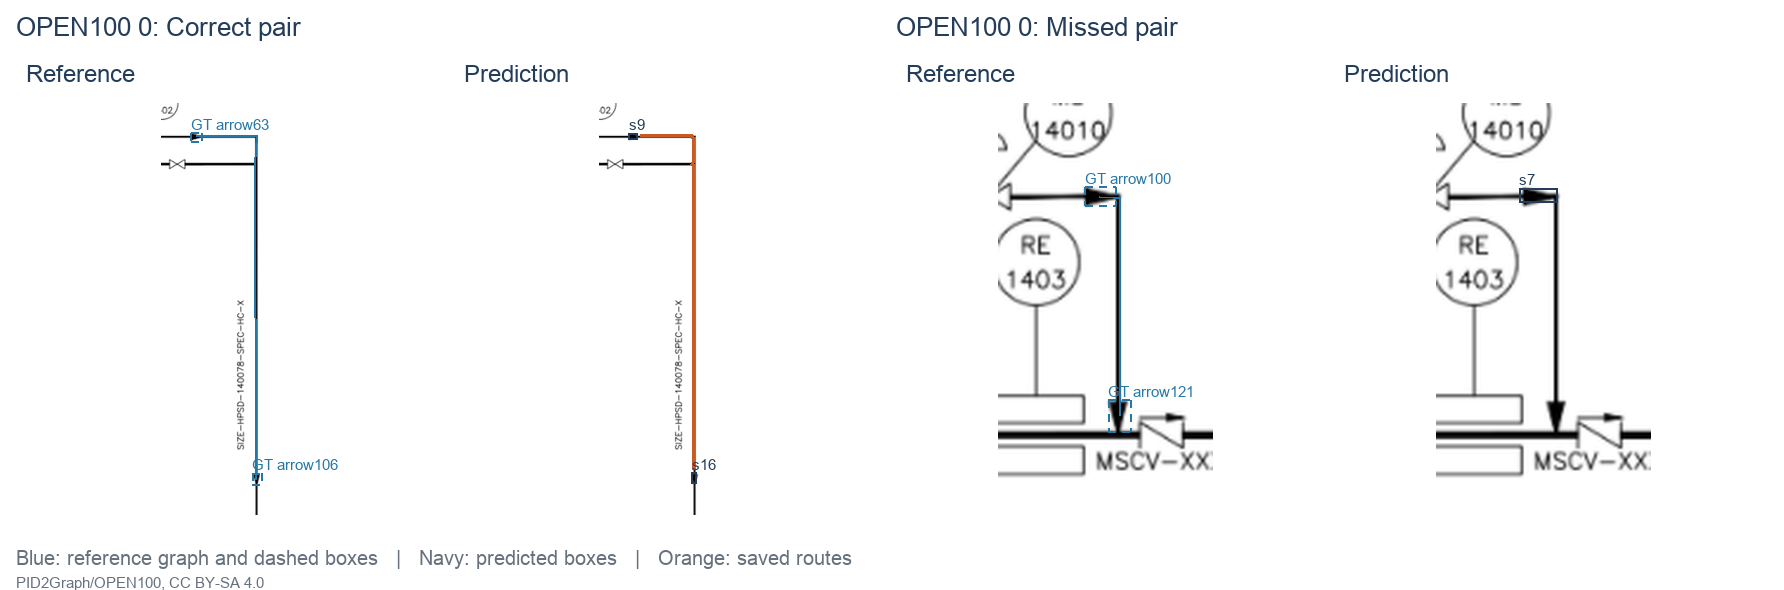
\includegraphics[width=\textwidth]{figures/open100_examples.png}
\caption{Actual OPEN100 original crops and saved v12 outputs: one correct and one missed pair, selected in fixed plan/pair order with a shared route-span legibility rule. Blue dashed boxes and center-joined paths are reference overlays; navy boxes and orange routes are predictions. References entered evaluation only; correctness denotes reference agreement, not improvement over v11. PID2Graph/OPEN100, CC BY-SA 4.0.}
\Description{Two public benchmark cases each compare an unchanged original crop with reference and saved prediction overlays. One pair is correctly extracted, while another reference connection is missed.}
\label{fig:benchmark}
\end{figure*}

\subsection{Evaluation Protocol}
The primary localization score considers every annotated physical symbol and every predicted non-text object. Native floating-point bounds remain unchanged; inclusive predicted maxima receive $+1$ for interval-area calculation. One-to-one matching first maximizes the number of pairs with box IoU $\ge .50$, then total IoU. Unmatched predictions are false positives and unmatched references are false negatives. Micro precision, recall and F1 pool counts across all plans. A separate class-aware diagnostic maps tanks and pumps to equipment; it does not replace class-agnostic localization.

For an adapted symbol-net reference, retain native symbol-to-symbol edges and collapse components induced by connector and crossing nodes. Add pairs among adjacent physical symbols, stopping traversal at another physical symbol. This yields 1,882 undirected reference pairs. Predictions use accepted-edge components separately within each exported net, as in Equation~\eqref{eq:reach}. Matching uses the fixed class-agnostic object assignment. Unmatched endpoints count as false positives or false negatives as appropriate. This score evaluates derived symbol-net connectivity, not PID2Graph's native node AP or edge mAP. Background regions, connector localization, edge types, text transcription and flow direction are not scored.

\begin{table}[t]
\centering
\caption{All 12 OPEN100 plans. Micro precision (P), recall (R) and F1 are percentages. Localization uses IoU $\ge .50$; connectivity is the adapted symbol-net score.}
\label{tab:benchmark}
\begin{tabular}{@{}llrrr@{}}
\toprule
Metric & Revision & P & R & F1\\
\midrule
Localization & v11 & 51.71 & 20.99 & 29.86\\
             & v12 & 51.71 & 21.06 & 29.93\\
Connectivity & v11 & 22.06 & 7.28 & 10.95\\
             & v12 & 22.49 & 7.01 & 10.69\\
\bottomrule
\end{tabular}
\end{table}

\subsection{Results and Preservation Failures}
V12 exports 586 symbols: 303 matched, 283 unmatched, and 1,136 references missed. Its 587 within-net pairs include 132 matches and 455 unmatched predictions, with 1,750 references missed. V11 exports 584 symbols and 621 pairs. Table~\ref{tab:benchmark} shows a 0.07-point localization F1 gain and a 0.25-point connectivity decrease. Shared caching and absent repeated-run uncertainty prevent causal or significance claims. The merged-class localization diagnostic yields 28.67\% F1 for v11 and 29.14\% for v12.

Strict correspondence uses unique identical class/box signatures across raw exports and checks their trace agreement. Of 2,908 old objects, including text, 2,856 map exactly; 52 do not. Only 2/12 plans pass the full object and relationship audit. Table~\ref{tab:preservation} separates mapped losses from relations incident to unmapped objects. Retaining reachability cannot excuse a missing direct edge, and unassigned endpoints cannot be counted as preserved. The raw v12 candidate therefore fails the preservation contract on ten plans. This is an offline audit result, not an accepted preservation-certified revision.

\begin{table}[t]
\centering
\caption{Strict v11$\to$v12 preservation across all plans. Lost counts only relations with mapped endpoints; unmapped relations are reported separately.}
\label{tab:preservation}
\begin{tabular}{@{}lrrrr@{}}
\toprule
Relation & Old & Retained & Lost & Unmapped\\
\midrule
Direct $E$ & 484 & 426 & 14 & 44\\
Containment $I$ & 143 & 142 & 0 & 1\\
Within-net $R$ & 621 & 511 & 57 & 53\\
\bottomrule
\end{tabular}
\end{table}



\subsection{Examples and Limitations}
Figure~\ref{fig:benchmark} illustrates source-linked decisions; all-plan metrics determine performance. Reference overlays enter evaluation only, and proposed connections are never painted into model verification views.

OPEN100 is a small related collection with solid reference edges. The prior study's 60 real training diagrams are private; our public legend does not reproduce its supervised regime, and hosted-model pretraining membership is unknown. Low recall and failed preservation limit transfer claims. P\&ID results do not establish CLD-rule gains. External comparisons, stochastic uncertainty, text transcription, cross-document links, RDF export and Web retrieval remain unmeasured or unimplemented.

\section{Conclusion}
The framework makes geometric and visual decisions inspectable and provides explicit tests of frozen-output preservation. On all 12 public OPEN100 plans, the candidate reaches 29.93\% localization F1 and 10.69\% adapted connectivity F1, with many missed symbols and links. Ten plans fail strict preservation. Original-pixel examples and separate audit counts expose these limits; they do not establish a general accuracy or repair guarantee.

\section*{Acknowledgement}
We acknowledge the contributors of PID2Graph and OPEN100 for making the benchmark available. Dataset attribution and usage conditions are recorded with the experiment artifacts.

\bibliographystyle{ACM-Reference-Format}
\bibliography{references}
\end{document}
